\section{Making a Monte Carlo integrator}


First, we explored different methods
in order to gain a better insight on how to create a better general integrator. We tested 4 methods, where each differs in how
the points in the domain are chosen to evaluate the integral.
The integration schemes \cite{MCmethods} used are:
\begin{enumerate}
  \item Uniform Static - The entire domain is divided by a uniform mesh were each point is taken in a coordinate is the grid.
  \item Uniform Adaptive - The domain is divided uniformly in square boxes, and for each box a mesh grid is created
  specified by a density value which determines the total number of points inside that box. The density parameter
  is obtained by performing successive iterations, on which the density of each sub-box is set by the total value of the integral inside
  the box.
  \item Stratified Static - The entire domain is divided in a uniform mesh, where for each quadrant of the mesh
  a single point is chosen randomly inside.
  \item Stratified Adaptive - Basically a combination of both methods adaptive and stratified.
\end{enumerate}

To compare each method we used a test function on which we evaluated the integrals.
This test function consisted on a donut shaped with value constant value in a 2-dimensional domain, from which
we can know the exact value of the integral easily. The results
of the error obtained for the different methods as a function of the number of points used is shown in fig. \ref{mc_errs},
 where 500 repetitions where used for each number of points and in the case of adaptive methods the entire integration
 domain was divided into 25 boxes. As
expected the best method is the adaptive stratified which has also gives the smallest standard deviation from the error as seen in the error bars.
Additionally is important to distinguish the steps in the error of the uniform static
method which are the systematic error introduced by the regular mesh. This shows the entire point of doing Monte Carlo integration!
\begin{figure*}[ht]
  \begin{center}
  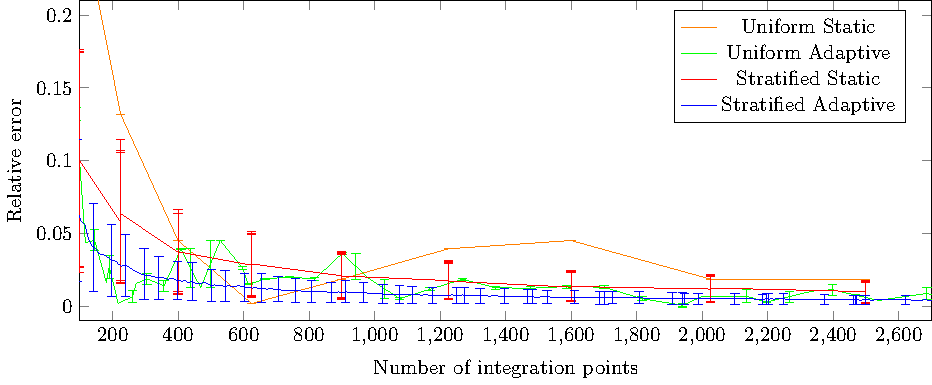
\includegraphics[scale=1 ]{graphs/integration_test_ring.pdf}
  \caption{Performance comparison of different numeric integration methods. The absolute value of the difference between the numerically calculated result and the analytical answer plotted against the number of integration points used. The used function is a two-dimensional ring (see text).}
  \label{fig:int}
  \end{center}
\end{figure*}
